Testing \& Consultancy Cell is a Department in our college that provide 
testing and Consultancy services to different clients. This cell does a 
lot of work like managing the clients, handling there work till 
completion. This work also requires managing a lot of paper work. 
Thus LibreHatti Software comes into the use. \\ 
{\bf Features of the Software}
\begin{itemize}
\item Open Source
\item User Interative Software
\item Online
\item Dynamic
\item Proper User and Admin interface
\item Catalog
\item Distance Calculation through map
\item Efficient Search module
\item Universal (Can be changed according to application/work)
\item Report generation
\item Single click installation
\item Proper User and develpor documentation
\end{itemize}

\newpage
{\bf Admin Interface}\\

The admin Interface is the Software interface for only admin. Using 
this interface admin can make all the changes in the Software. He/She 
is the utmost authority. The services that are given to the end user 
can be added, updated or deleted by the admin. Admin is the one who 
gives the permission for certain authority of a User.\\ 
\begin{figure}[h]
\centering 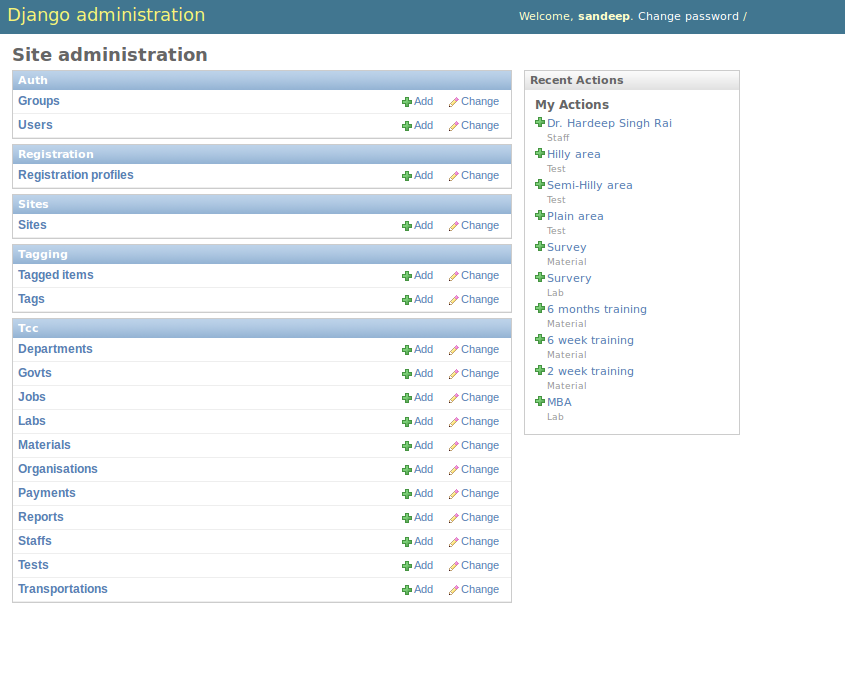
\includegraphics[scale=0.6]{images/admin.png}
\caption{Admin Interface}
\end{figure}

\newpage
{\bf Welcome Screen}\\

This Welcome Screen is visible as soon as the link to the Software is 
opened. This screen is visible to all the users even if they are 
authenticated or not.
\begin{figure}[h]
\vskip 2cm
\centering 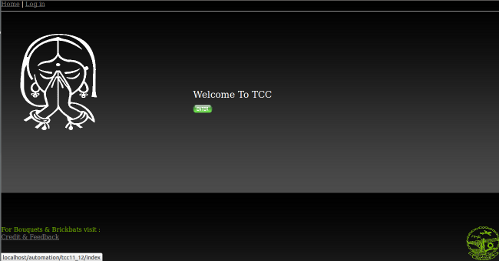
\includegraphics[scale=1.0]{images/welcome.png}
\caption{Welcome Screen}
\end{figure}

\newpage 
{\bf Registration \& Login}\\

When a User tries to login into the Software, the software checks, 
whethere the user is valid or is authenticated. If yes, the user login 
into the Software is susccesfull, else the User need to register 
himeself as the User.As soon as the user register himself, he will be 
sent an activation mail. In order to activate the account, the user 
has to open that link and login himself. Only the authenticated user 
is able to use the features of the software or work with it.
\begin{figure}[h]
\vskip 2cm
\centering 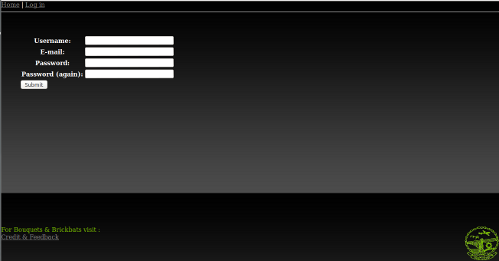
\includegraphics[scale=1.0]{images/register1.png}
\caption{Registration Screen}
\end{figure}

\newpage
{\bf Employee Login}\\
 
An employee is the User who has the authority to register other 
clients into the Software and then add there jobs or manage them. Once 
an authenticated employee login into the system, he/she is able to use 
all the fuctionality availble to him/her. He can add the clients, handle 
them, see the wotk of all the clients. A lot of features are availaber 
for the employer to automate his work and make it easy.
\begin{figure}[h]
\vskip 2cm
\centering 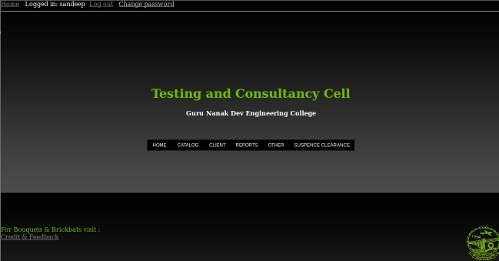
\includegraphics[scale=1.0]{images/user1.png}
\caption{Employe Interface}
\end{figure}
\newpage
{\bf Normal User Login}\\

A normal User is considered as the client. He has very limited acess on 
the features of the software. In LibreHatti Software, the users 
have different web interface of the Software depending on the authority 
they are given. A normal User can have the information about all the 
services available, ask for a service, thus registering what actually 
he wants. He can also see the previous services he used from the Cell. 

\begin{figure}[h]
\vskip 2cm
\centering 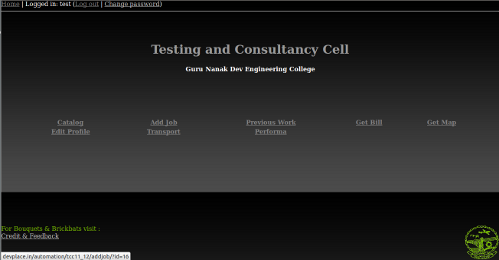
\includegraphics[scale=1.0]{images/user2.png}
\caption{Normal User Interface}
\end{figure}
\newpage
{\bf Catalog}\\
Catalog provides all the information about the product, there rate, 
quantity etc. Seeing the catalog list user can get an estimate of the 
total amount he would spend on entering a Job or work. A catalog 
represents a collection of products that you group into categories. 
You can then use this information to create, within a Commerce 
Server-enabled Web site, Web pages that let your customers browse your 
collection of products. The categories in your catalogs can have 
sub-categories, and products may appear in multiple categories.\\


\begin{figure}[h]
\centering 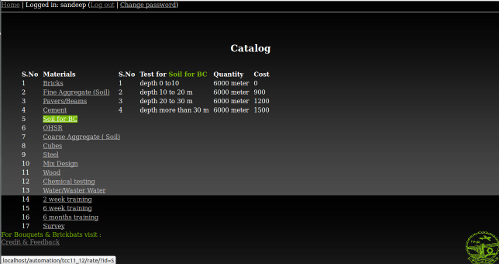
\includegraphics[scale=1.0]{images/Catalog.png}
\caption{Catalog}
\end{figure}

Catalogs contain hierarchies and relationships that you use to organize 
the products in the catalog to make it easier for customers to navigate 
to the products that they want to buy. You can create category 
hierarchies and relationships among categories and products that are 
in the same catalog or in different catalogs. For example, if you have 
a large catalog, you can create a parent category that includes several 
other categories, known as child categories. When customers navigate to 
the parent category, the child categories appear; enabling customers to 
navigate quickly to the category that contains the products they want.
\newpage
{\bf Add Job}\\

Both employee and Normal User can add the Job. The only difference is 
that an employee can add multiple jobs for his different clients and 
normal user can add the jobs for only himself. For adding the job one 
needs to fill all the necessary data required for a work to be done.
All the calculations about the amount for the Job is done in the backend. 
Only after you click the submit button you will be able to see the 
results.
\begin{figure}[h]
\vskip 2cm
\centering 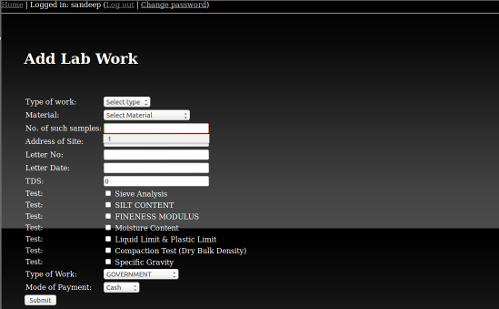
\includegraphics[scale=1.0]{images/addjob1.png}
\caption{Add Job Form}
\end{figure}

\newpage
{\bf Search Module}\\

The search module include searching a client or Job that has previously 
been added. After getting the results of the search, the operations 
like getting the previous work done by the client, status of those works 
or further adding new works are performed. It is an important feature 
of the software as it keeps the track of the clients getting services 
from the organisation.

\begin{figure}[h]
\vskip 2cm
\centering 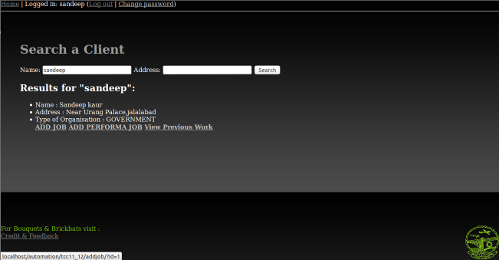
\includegraphics[scale=1.0]{images/search1.png}
\caption{Search Module}
\end{figure}
In this, the Software looks for the certain keyword you entered in the 
corresponding table. The filteration is done and those results with 
matching keywords are listed. 

\newpage
{\bf Bill, Receipt \& Voucher generation}\\

Once the Job is entered into the software, irrespective of when it will 
start, the client is required to make the payment. After that he is given 
the Receipt and bill for his work. The Bill, Receipt and Voucher are 
automatically generated only after a complete and valid Job is added 
into the software.
\begin{figure}[h]
\vskip 2cm
\centering 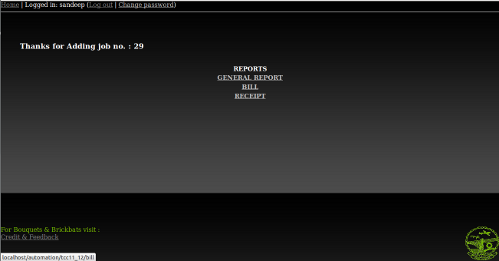
\includegraphics[scale=1.0]{images/Bill.png}
\caption{Get Bill, Receipt \& Voucher}
\end{figure}

\newpage 
{\bf Registers Generation}\\

This module involves retrieving all the previous entries that were 
performed. These registeres include : Daily Report, Monthly Register, 
Main Register, Suspence Clearance Register, Lab Report, Client Report 
etc. For getting different registers diffeent queries are performed or 
filter are applied, depending on the need.\\
\begin{figure}[h]
\centering 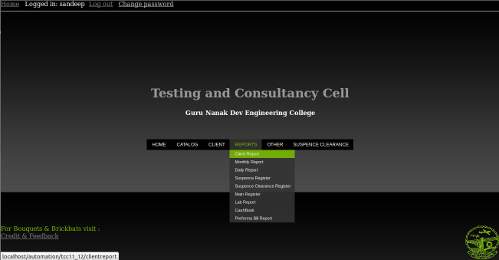
\includegraphics[scale=1.0]{images/registers.png}
\caption{Select the Register}
\end{figure}\\
{\bf Registers generated in the software}\\
Following are the reports generated in LibreHatti software :
\begin{itemize}
\item Suspence Report: This report keep record of all the suspence 
jobs that has been registered.
\item Suspence-Clearance Report: This report is used to get all te 
suspence registered jobs whose dues have been cleared out.
\item T.A./D.A. Bill: This is report for Transport Allowance and Daily 
Allowance bill.
\item Performa Bill: It give the 
\item Job Register: It keep record of all the jobs registered.
\item Yearly/Monthly Income Report: It gives the yearly and monthly 
record of income to the institute.
\item Transport Bill: It gives all the information related to 
transportation.
\item Other charge Bill: It gives the report of all the other charges 
like service tax, education tax, etc.
\item Daily report: It gives the information of job registered in  the 
number of days selected. It also makes the differance between the types 
of payments made like cheque, cash.
\item Faculty Income distribution: It keeps the record of the income 
distribution to the faculty members.
\item Main Register: It is the main register keeping the record of all 
the report types.
\item Receipt: It keeps te record of all the recieps. One only need to 
know the job no. and then can easily get the receipt.
\item Department/lab Report: It carries all the information of various 
labs and thus gives the record for the lab selected.
\item Govt./Semi-Govt./Private Report: It keeps the record for the type 
of work selected i.e Govt./Semi-Govt./Private Report.
\item Clearance Report: It gives the clearance report.
\item General Bill: It keeps record of all the general reports.
\end{itemize}

\begin{figure}[h]
\centering 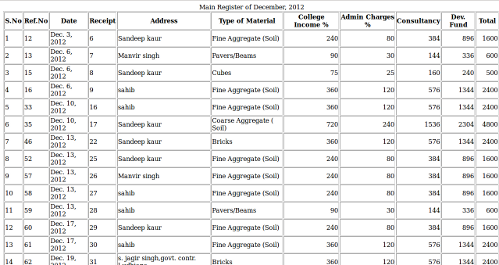
\includegraphics[scale=1.0]{images/reg1.png}
\caption{Output Register}
\end{figure}

\newpage
{\bf Report Generation}\\

Report Generation module include generating the complete report for the 
field work.This gives the detailed information about the work done, 
staff mebers involved in doing the work, calculations done etc. 
Multiple Reports re generated for a work done from different labs. 
Once the report is generated one can download it too. Now the basic 
requirement of the project  is to produce the report from the the data 
which were submitted by the user or client in the office for the 
testing purpose. So, for that we require the generic views for the 
software to display the data from the models of the report and to 
display that data to the user we also need the templates for the 
different types of the reports. It is necessary for the report 
application that the templates for the report application must be 
different from the other application templates so that it is easily 
distinguished from the tcc application which was another application 
in the project. So, for this purpose the different template inside the 
templates of the project was made to distinguish the different template. 
This template is known as ``report".\\\\
The reports are generated from the models which are predefined in the 
models of the report application, In the  models field, there are 
different types of field which are responsible for storing the data in 
the different datatypes. The good thing is that we can distinguish 
between the tables of the two applications very easily, as the prefix 
for the different applications are set by default by the the syncdb 
process. And in this case, the models are made with the prefix 
``report".\\\\
\begin{figure}[h]
\centering 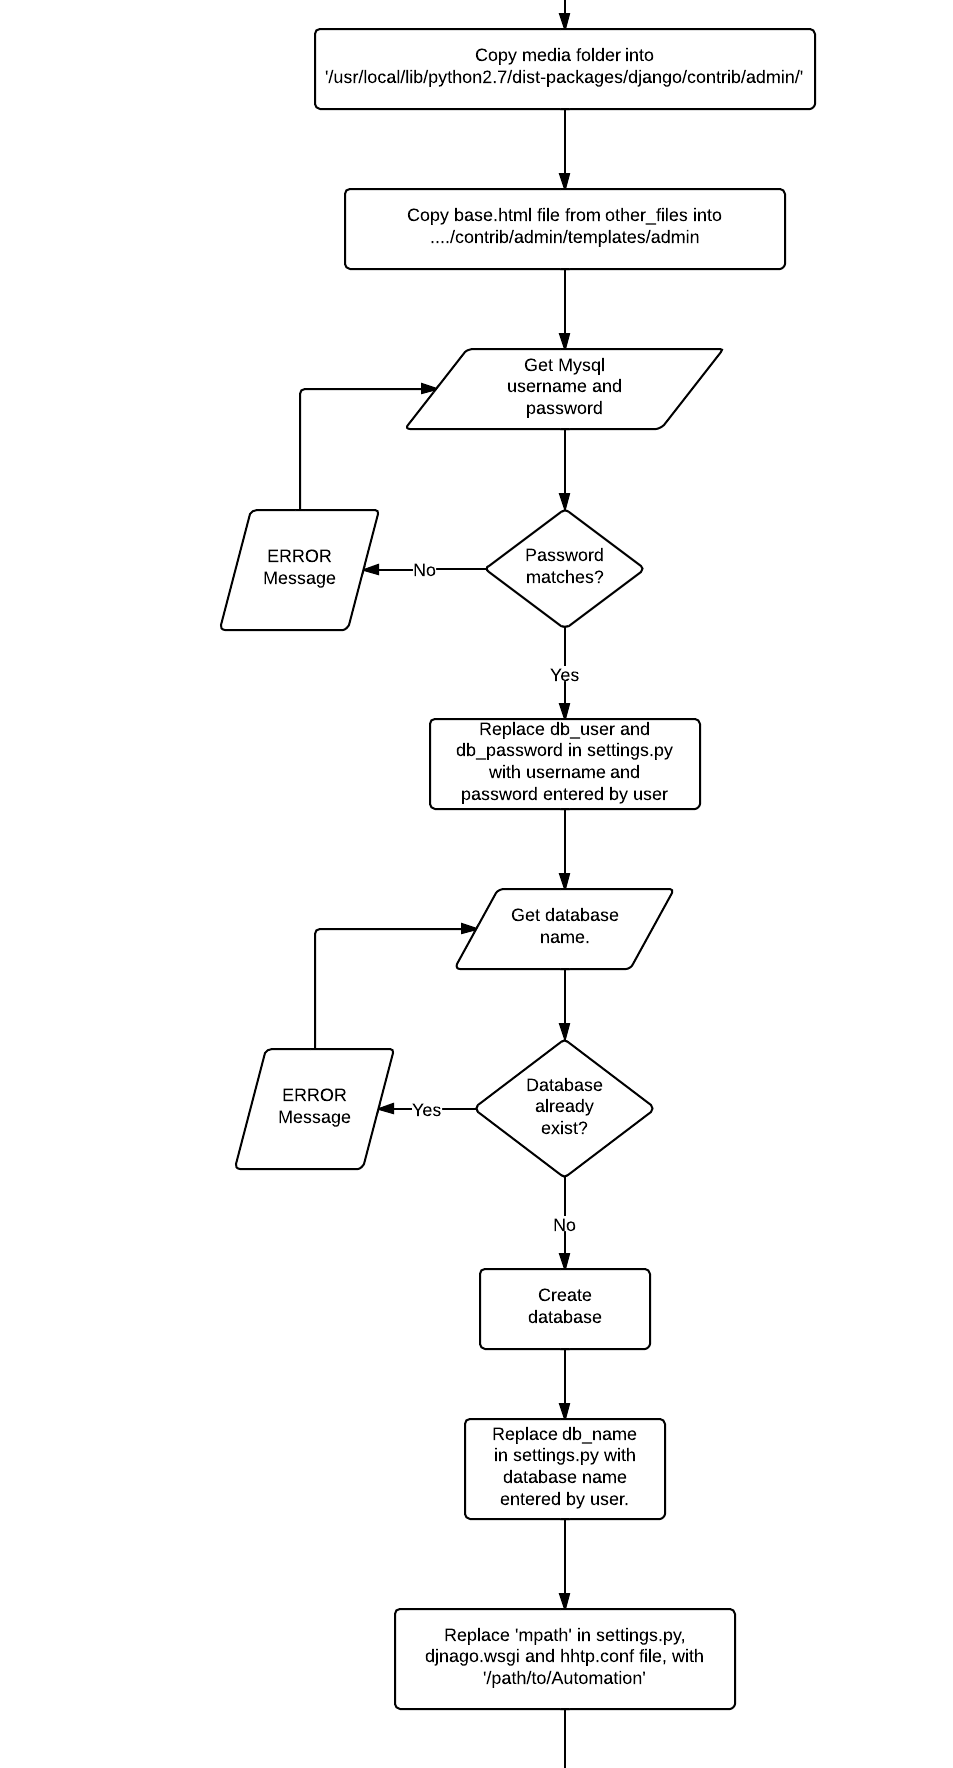
\includegraphics[scale=1.0]{images/inst3.png}
\caption{Types of Report}
\end{figure}
SELECTING THE TYPE OF REPORT FROM THE GIVEN MATERIAL :\\\\
To make the report one should need to select the type of report which 
the user want to produce, so for this purpose the report type has to 
be chosen from the list of the available report in the software. The 
report formats are directly called from the models via views and a 
common form.html is responsible for displaying the form.\\\\
On clicking any of the report the specific report is selected and we 
can proceed further to fill the entries into that report.\\\\
SELECTING AND MAKING A SPECIFIC REPORT TYPE\\\\
At this step, the selected report form is displayed in front of the 
user and now the user can fill the data which he can attain from the 
lab after testing the different material, there might be the different 
samples of the same material, at the top of the form a column for 
specifying the sample no is given in the form, the form them contains 
the different fields according to the requirement of the material and 
test. All the fields are predefined according to the different tests, 
so the user only have to fill the test values in the form.\\\\
FINAL REPORT\\
The final report is produced by clicking on the submit button on the 
form in the report type to be added. The sample of the report is 
attached below: 
\newpage
\begin{figure}[h]
\centering 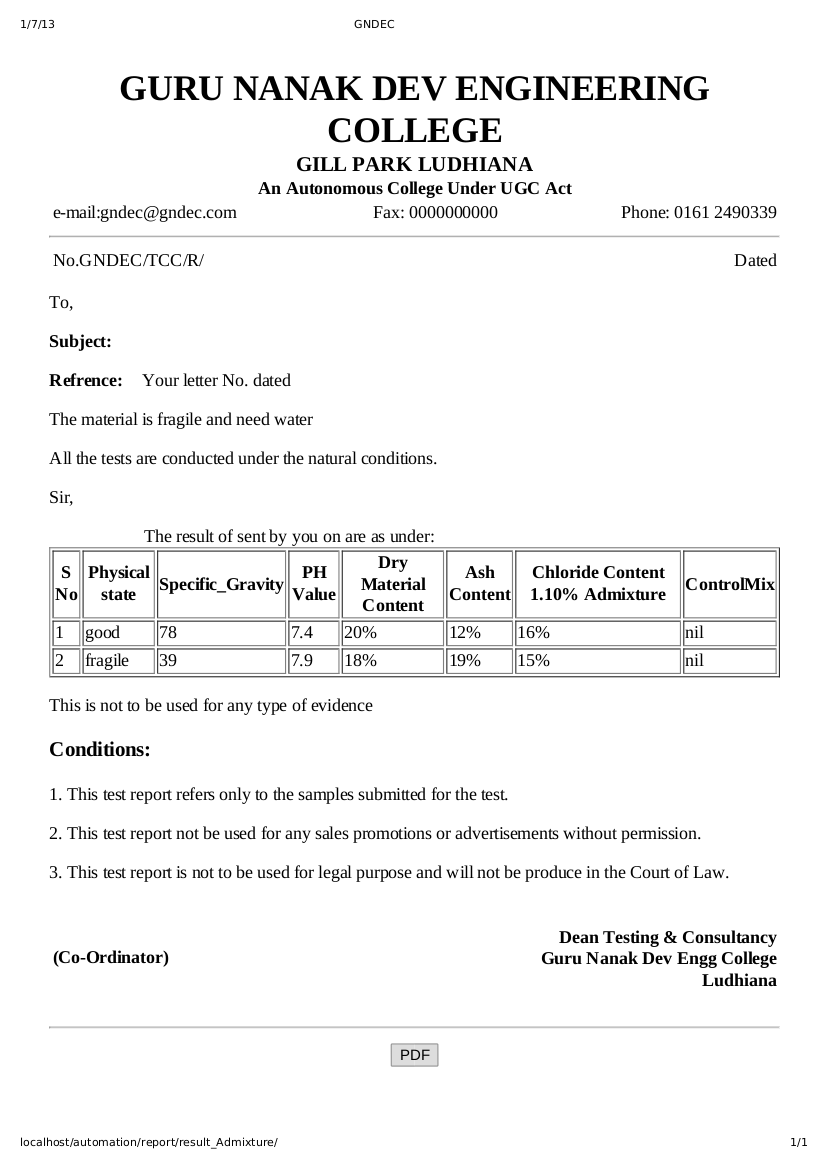
\includegraphics[scale=0.1]{images/GNDEC.png}
\caption{Report Generated}
\end{figure}




\newpage
{\bf Distribution of money}\\

\begin{itemize}
\item College Income
\item Administrative
\item Development Funds
\item Consultatancy Asst.
\item Service Tax
\item Education Tax
\item Higher-Education Tax
\end{itemize}
